\documentclass[11pt,a4paper]{article}
\usepackage{tipa}
\usepackage{emoji}
\usepackage{pdfpages}
\usepackage[utf8]{inputenc} % Zeichenkodierung
\usepackage[T1]{fontenc}    % Bessere Zeichenunterstützung
\usepackage[german]{babel}  % Korrekte deutsche Typografie
\usepackage[a4paper, left=2cm, right=2cm, top=2.5cm, bottom=2.5cm]{geometry}
\usepackage{amssymb, amsmath, amsthm}
\usepackage{tikz}
\usepackage{graphicx}
\usepackage[export]{adjustbox}
\usepackage{microtype}
\usepackage{epstopdf}
\usepackage{float}
\usepackage{amsmath}
\usepackage{amssymb}
\usepackage{amstext}
\usepackage{amsfonts}
\usepackage{mathrsfs}
\usepackage{hyphenat}
\usepackage{fancyhdr}  
\usepackage{amsmath, amssymb}
\usepackage{graphicx}
\usepackage{graphicx}   % Zum Einbinden von Bildern
\usepackage{wrapfig} 
\usepackage{pgfplots} % Für das Zeichnen des Signals
\pgfplotsset{compat=1.18}
\usepackage{qrcode}  % QR-Code generieren
\setlength{\skip\footins}{40pt}
\title{}
\date{}  % Kein Datum auf Standard-Titel

\begin{document}

% === DECKBLATT ===
\begin{titlepage}
    \centering
    
    {\Huge Netzwerke und Schaltungen II}\\[0.8cm]
    {\Large D-ITET}\\[0.8cm]
    {\Large HS2025}\\[3.5cm]
    
    {\Huge \textbf{Übung 1}}\\[1cm]
    {\Large 21.2.2025}\\[3.5cm]

    \qrcode[height=6cm]{https://n.ethz.ch/~rsahleanu/nus2/}

    \vfill
    {\Large \textbf{Rares Sahleanu}}
\end{titlepage}

% === INHALTSVERZEICHNIS ===
%\newpage
%\tableofcontents

% === AKTIVIERT KOPF- UND FUSSZEILEN AB SEITE 3 ===
\newpage
\pagestyle{fancy}  

% Kopfzeile: Links - Mitte - Rechts (subtil & kleiner)
\fancyhead[L]{\small \textit{Netzwerke und Schaltungen II}}  
\fancyhead[C]{\small \textit{Übung 1}}
\fancyhead[R]{\small \textit{Rares Sahleanu}}

% Fußzeile: Seitenzahl in der Mitte
\fancyfoot[L]{}  
\fancyfoot[C]{\thepage}
\fancyfoot[R]{}

% Linie in der Kopfzeile aktivieren, Fußzeile ohne Linie
\renewcommand{\headrulewidth}{0.4pt}  
\renewcommand{\footrulewidth}{0pt}  

% === START DES DOKUMENTS ===
\section{Organisatorisches}
Kurz zu mir: Ich heiße Rares\footnote{ausgesprochen \textit{Raresch} \textipa{['ra:r\esh]}}, bin 19 Jahre alt und sitze mein 4. Semester am ITET ab. Zu meinen größten Errungenschaften gehören der Rank \textit{Distinguished Master Guardian} in CS:GO, eine aufstrebende Hobby-Rapper\footnote{Man kennt mich unter einer Vielzahl von Künstlernamen: LilReez, LilReezy, RaresDerAgrarmensch, Reez} \textit{Karriere und +6.00 CHF} Endbilanz bei swisslos.ch\footnote{Sportwetten sind nicht meins. Meistens wettet der ``Zug-Typ'' Eddy, und ich nehme die Rolle der Opposition ein, indem ich seine Entscheidung runterrede}. 

\subsection{FAQ}
Hier ist eine Liste der Fragen, die oft gestellt werden:

\subsubsection{``Wie ist das Fach XY{?}``}
Im zweiten Semester liegt die Schwierigkeit weniger in der \textit{Komplexität} des Stoffes, sondern mehr in der Menge. Es ist VIEL STOFF, aber dafür ist er nicht allzu ``schwer`` zu verstehen. Ach und: Wenn man nicht programmieren kann bzw. keine Vorerfahrungen in Informatik hat, dann sollte man Informatik sehr, sehr, sehr ernst nehmen. Hier eine kleine Übersicht:

\begin{itemize}
    \item \textbf{Analysis 1/2}: Am Ball bleiben und Serien lösen! Besonders Ziltener hält sich sehr nahe an den Serien, und seine Klausuren sind fair. Die Prüfung geht ``nur`` 4 Stunden, und da kann er nicht alles abfragen. Es kommen nur Key-Concepts dran, welche man gut üben kann.
    \item \textbf{Komplexe Analysis}: Ein ``normaler`` Kurs. Es lässt sich alles gut grafisch vorstellen, und die Aufgaben in der Klausur sind sehr ``absehbar``. Unterschätzen sollte man es nicht, aber zu viel Zeit investieren auch nicht.
    \item \textbf{Physik}: Inhaltlich hält es sich sehr nah an den anderen Fächern. Schwingungen sind basically eine Carbon-Copy von den anderen Fächern. Gut ``übbar`` und mit Notenbonus ist die Klausur machbar.
    \item \textbf{Informatik}: Squid-Game in Reallife. Wenn man programmieren kann, dann easy. Wenn nicht, dann ist es ein ernstzunehmendes Fach, sonst wirklich Krise. Hier gilt: Üben, üben, üben.
    \item \textbf{Netzwerke und Schaltungen}: Neben Analysis das wichtigste Fach. Der Stoff hält sich in Grenzen\footnote{Wie Adventskerzen – fragt gerne, falls ihr das nicht verstanden habt}, aber in der Klausur wird hauptsächlich Schnelligkeit und Routine abgefragt. Wer viel übt, holt in der Regel gute Noten.
\end{itemize}

\subsubsection{``Was kannst du zum Üben empfehlen{?}``}
Für Informatik empfehle ich ganz klar die C++-Bibel\footnote{ISBN-13: 978-3836298537} von Thorsten Will in Kombination mit LeetCode und den TA Maximilian Hoh\footnote{https://n.ethz.ch/~mhoh01/index.html}. Für Analysis ist es zu 100\% der TA Angelo Nujic\footnote{https://polybox.ethz.ch/index.php/s/UxNajbQ3tLOh4pH} und die Übung. Für NuS lege ich euch die Probeprüfungen ans Herz. Die Prüfung ist immer dieselbe, weshalb sich Üben mit den Probeprüfungen lohnt!

\subsubsection{``Ich habe in Analysis 1 nicht ganz aufgepasst – ist das schlimm{?}``}
Nein. Ich war selbst nur in den ersten beiden Vorlesungen von Analysis 1 und habe mir vereinzelt Aufzeichnungen angeschaut und ca. 30\% der Serien gemacht. In Analysis 2 wird eh alles neu aufgerollt.

\subsubsection{``Ich bin in BP A gerade so durchgekommen. Ist das ein Problem{?}``}
Entgegen aller Gerüchte ist das 2. Semester nicht komplizierter, sondern nur schwer. Was zuerst paradox wirkt, bedeutet, dass man nur viel zu tun hat, aber es gibt keinen Stoff mehr, den man etwas nicht mehr versteht, weil es keinen Sinn macht.

\subsection{Overview Übungsstunde}
\centering

% Erster Eintrag
\begin{minipage}{0.8\linewidth}
    Website der Übungsgruppe
    \hfill  
    \qrcode[height=4cm]{https://n.ethz.ch/~rsahleanu/}
\end{minipage}

\vfill % Gleichmäßiger Abstand zwischen den Einträgen
\begin{minipage}{0.8\linewidth}  
    Whatsapp-Gruppe
    \hfill  
    \qrcode[height=4cm]{https://chat.whatsapp.com/JprzBOwpTco32ea71sphA3}
\end{minipage}
\vfill
\begin{minipage}{0.8\linewidth}
    Umfrage zum Format
    \hfill  
    \qrcode[height=4cm]{https://forms.gle/iwhNmMewyoqQw2HaA}
\end{minipage}

\raggedright
\subsection{Zusätzliches}
Die Übungsstunde wird, soweit möglich, aufgezeichnet. Fragen beantworte ich gerne über Whatsapp, Discord, Email. Wenn jemand etwas an dem TeX-Template ändern möchte soll er einfach eine Merge-Request machen. Ideen zur Website gerne mir schicken :))
\newpage
\subsection{Für unseren Kurs}


\begin{itemize}
    \item \textbf{Bonus}: Den Bonus bekommt ihr, indem ihr wöchentlich die Aufgaben löst und sie abgebt. Dabei sind die Aufgaben und nicht die „Zusatzaufgaben“ gemeint. Der Notenbonus wird ab 50\% vergeben und linear bis maximal 75\% der Punkte verrechnet.
    \item \textbf{Wochenablauf}: Woche N: Bis zur Übung soll man sich die Videos von Woche N\footnote{Slide 9 in den „Lectureslides“} anschauen und, sofern man Zeit hat, sich einmal in die Übung eindenken. Anschließend hat man dann eine Woche (ab der Übung) Zeit, um die Übung zu lösen und abzugeben.
    \item \textbf{Taschenrechner}: Ich empfehle den „TI-Nspire CX II CAS“.
    \item \textbf{Prüfungstipps}: Die Prüfung hat immer denselben Aufbau, weshalb es sinnvoll ist, sich einige Automatismen anzueignen. Aufgabe 1 lässt sich „auswendig lernen“ und Aufgabe 4 kann mit etwas Glück\footnote{Erkläre ich, wenn es soweit ist.} vereinfacht werden. Aufgabe 3 kann man mit Übung sehr schnell lösen.
    \item \textbf{Empfohlene Lernmittel}: 1. Videos 2. Skript 3. Buch (Albach) 4. Die „anderen“ Bücher.
    \item \textbf{Nützlich}: Nutzt LTSpice und Falstad\footnote{https://falstad.com/circuit/circuitjs.html}
    \item \textbf{Letzter Tipp}: Macht einfach die Probeklausuren, bis ihr auswendig wisst, was die Lösungen sind und ihr seid sicher. 
\end{itemize}


\begin{figure}[h]
    \centering
    \begin{minipage}{0.3\textwidth}
        \centering
        
\includegraphics[width=\textwidth]{memes/meme1.jpg}
    \end{minipage}
    \begin{minipage}{0.3\textwidth}
        \centering
        
\includegraphics[width=\textwidth]{memes/meme2.jpg}
    \end{minipage}
    \begin{minipage}{0.3\textwidth}
        \centering
        
\includegraphics[width=\textwidth]{memes/meme3.jpg}
    \end{minipage}
\end{figure}

\newpage
\raggedright
% === ZWEITES KAPITEL ===
\section{Effektiv- und Scheitelwert}
Soooo, fangen wir erstmal mit den Basics an :) Bevor es so richtig losgeht, müssen wir aber erstmal ein paar Definitionen machen.

\subsection{Scheitelwert/Spitzenwert}
Der Scheitelwert ist einfach der maximale Wert, den eine Schwingung erreicht.

\subsection{Periodendauer/Frequenz/Winkelfrequenz}
Die Periodendauer einer Frequenz gibt an, ``wie lange`` es dauert, bis sich die Schwingung wiederholt. Die Frequenz ist dementsprechend
\[
\frac{1}{T}
\]
und gibt an, wie oft pro Sekunde sich eine Schwingung ``wiederholt``. \\
\( \rightarrow \) Die \textit{Winkelgeschwindigkeit} \( \omega=\frac{2\pi}{T} = 2\pi f \) ``mappt`` das Signal zuerst auf einen Kreis und gibt an, ``wie schnell`` man sich drehen muss, um das Signal korrekt zu lesen.

\subsection{Mittelwert/Gleichrichtwert/Effektivwert}
Um Wechselspannung zu beschreiben, benötigen wir einige \textit{repräsentative} Werte, die aber – Gott sei Dank – alle intuitiv sind :)

\begin{itemize}
    \item \textbf{Mittelwert}\footnote{In der Klausur ist so etwas i.d.R. immer gleich 0. Man kann hier oft Symmetrien ausnutzen} \quad \( \bar{u} = \frac{1}{T} \int_{t=t_0}^{t=t_0+T} u(t) \, dt \rightarrow \) Fläche unter dem Graphen über eine Schwingung.
    
    \item \textbf{Gleichrichtwert} \quad \( |\bar{u}| = \frac{1}{T} \int_{t=t_0}^{t=t_0+T} |u(t)| \, dt \rightarrow \) Die Fläche unter dem Graphen, wenn man die negativen Anteile nach ``oben klappt``.
    
    \item \textbf{Effektivwert}\footnote{Bei \( \sin \) oder \( \cos \) kann man Symmetrien ausnutzen} \quad \( U = \sqrt{\frac{1}{T} \int_{t=t_0}^{t=t_0+T} u(t)^2 \, dt} \rightarrow \) Gibt an, welche Gleichspannung dieselbe Leistung liefern würde.
\end{itemize}


\section{Zeigerdarstellung}
Wir werden in NuS II hauptsächlich mit Zeigern arbeiten. Diese dienen als Brücke zwischen unserer echten Welt mit realen Zahlen und den komplexen Zahlen. Obwohl es ggf. zu Beginn nicht so scheint, erleichtern uns letztere das Leben :)

\subsection{Euler'sche Formel}
Jede mathematische Entdeckung wird immer nach dem zweiten Entdecker benannt. Wieso? Weil der erste immer Leonhard Euler\footnote{Neben einem funktionierenden Bahnsystem und ``El Tony``-Mate wahrscheinlich das Beste, was die Schweiz jemals hervorgebracht hat, war.} war. Danach ist unter anderem folgende Formel benannt.

\theoremstyle{definition}
\newtheorem*{definition}{Satz}
\begin{definition}
Sei \( \varphi \) ein Winkel, so gilt:
\[
\cos(\varphi) + j \sin(\varphi) = e^{j\varphi}
\]
wobei \( j \) die ``imaginäre Einheit`` ist. Sie ergibt sich aus \( j = \sqrt{-1} \).
\end{definition}

\noindent Das können wir nun mithilfe von ein paar Konventionen für unsere schwingenden Signale nutzen.

\subsection{Von der Schwingung zum Zeiger}

Nehmen wir nun an, dass eine Schwingung sinusförmig ist. So lässt sie sich schreiben als:
\[
u(t) = \hat{u}\cos(\omega t + \varphi) = Re\{\hat{u}e^{j\omega t + j\varphi}\} = Re\{\hat{\underline{u}} e^{j\omega t}\}
\]
mit \( \hat{\underline{u}} = \hat{u} e^{j\varphi} \), welcher der sog. ``Zeiger``\footnote{Der Drehanteil \( e^{j\omega t} \) ist für uns meist nicht von Bedeutung. Das wird aber während der Vorlesung klarer. Der Zeiger enthält nur Informationen über den Betrag und die Phase („Offset“). Die Idee ist, dass wir damit rechnen, die Schwingung ignorieren und sie am Ende wieder einrechnen.}
 ist.
\vspace{0.3cm}

Das kann am Anfang etwas verwirrend sein. Versucht es euch vorzustellen wie einen rotierenden Pfeil, der von oben mit Licht bescheint wird. Um die Schwingung zu erfassen, müssen wir nur den Schatten ablesen.

\centering 
\begin{figure}[H]
  \centering
  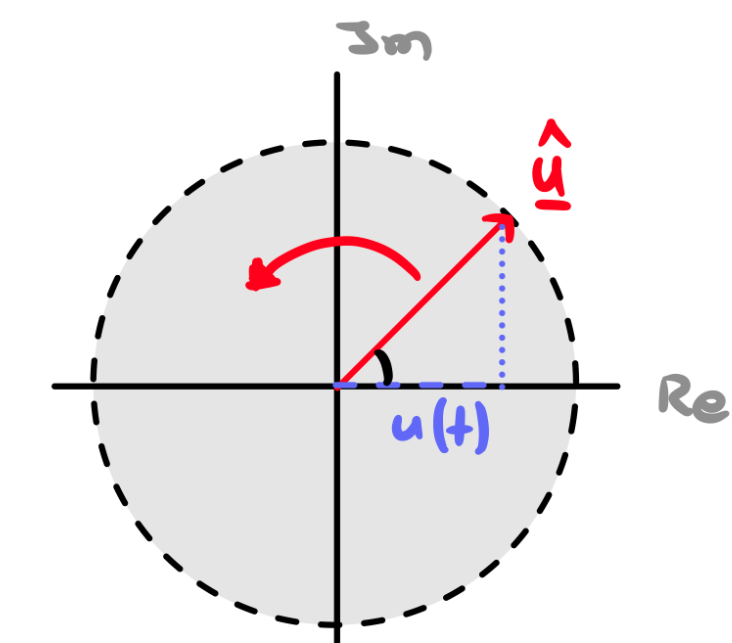
\includegraphics[width=0.4\textwidth]{pointer.png}
  \caption{Projektion des Zeigers}
  \label{fig:pointer}
\end{figure}
\centering

\raggedright



\subsection{Nutzen}
Zeiger bilden einen eigenen Raum. Das heißt, wir können Schwingungen eindeutige Zeiger zuweisen und umgekehrt. Ebenfalls gilt in diesem Raum das Distributiv-, Assoziativ- und Kommutativgesetz. Kurz gesagt: Um zwei Schwingungen zu addieren, können wir einfach deren Zeiger addieren und dann zurück ``wandeln``. Das gilt auch bei anderen Operationen. Hier eine Übersicht:

\begin{itemize}
    \item \textbf{Addition von Schwingungen:} \quad 
    \[
    a(t) + b(t) \quad \rightarrow \quad (\hat{\underline{a}} + \hat{\underline{b}}) e^{j\omega t}
    \]

    \item \textbf{Multiplikation mit einer Konstanten:} \quad 
    \[
    c \cdot a(t) \quad \rightarrow \quad (c \cdot \hat{\underline{a}}) e^{j\omega t}
    \]

    \item \textbf{Differenzbildung:} \quad 
    \[
    a(t) - b(t) \quad \rightarrow \quad (\hat{\underline{a}} - \hat{\underline{b}}) e^{j\omega t}
    \]

    \item \textbf{Skalierung von Amplituden:} \quad 
    \[
    k \cdot a(t) \quad \rightarrow \quad (k \cdot \hat{\underline{a}}) e^{j\omega t}
    \]

    \item \textbf{Phasenverschiebung:} \quad 
    \[
    a(t + \tau) \quad \rightarrow \quad \hat{\underline{a}} \cdot e^{j\omega \tau}
    \]

    \item \textbf{Modulation (Multiplikation mit einer anderen Schwingung):} \quad 
    \[
    a(t) \cdot \cos(\Omega t) \quad \rightarrow \quad \frac{\hat{\underline{a}}}{2} \left( e^{j(\omega+\Omega)t} + e^{j(\omega-\Omega)t} \right)
    \]

    \item \textbf{Differentiation im Zeitbereich:} \quad 
    \[
    \frac{d}{dt} a(t) \quad \rightarrow \quad j\omega \cdot \hat{\underline{a}} \cdot e^{j\omega t}
    \]
 
    \item \textbf{Integration im Zeitbereich:} \quad 
    \[
    \int a(t) dt \quad \rightarrow \quad \frac{\hat{\underline{a}}}{j\omega} e^{j\omega t}
    \]
\end{itemize}
\vspace{1cm}
$\rightarrow$ Das Ohm'sche Gesetz gilt auch im Zeiger-Bereich. Das heißt man kann einen ``Strom-Zeiger`` mit einem Widerstandswert multiplizieren und erhält den dazugehörigen ``Spannungszeiger``



\newpage
\section{Aufgaben}
\subsection{Komplexe Zahlen}
\begin{enumerate}
    \item \textbf{Betrag und Phase berechnen:}  
    Gegeben ist die komplexe Zahl:  
    \[
    z = 3 + 4i
    \]
    Berechne den Betrag \( |z| \) und die Phase \( \arg(z) \) in Grad.

    \item \textbf{Multiplikation und Division:}  
    Berechne die folgenden Operationen mit komplexen Zahlen:  
    \[
    (2 + 2i) \cdot (1 - i) \quad \text{und} \quad \frac{6 + 8i}{2 + 2i}
    \]
    Schreibe das Ergebnis in der Form \( a + bi \).

    \item \textbf{Komplexe Zahl in Polardarstellung umwandeln:}  
    Gegeben ist die Zahl:
    \[
    z = -4 + 4i
    \]
    Bestimme die Darstellung in Polarkoordinaten \( z = r e^{j\theta} \) mit \( r \) als Betrag und \( \theta \) als Phase in Grad.

    \item \textbf{Einzeichnen in die gaußsche Zahlenebene:}  
    Zeichne die folgenden komplexen Zahlen in ein Koordinatensystem ein:  
    \[
    z_1 = 1 + i, \quad z_2 = -2 + 3i, \quad z_3 = -3 - 4i
    \]
    Markiere sie mit ihren Koordinaten und dem jeweiligen Winkel zur positiven Realachse.

    \item \textbf{Wurzel einer komplexen Zahl:}  
    Berechne die beiden Lösungen von:
    \[
    \sqrt{5 + 12i}
    \]
    Schreibe die Lösungen in der Form \( a + bi \).
\end{enumerate}
\subsection{Nützliches}

Gegeben ist das Signal:
\[
x(t) = \sin(\omega t)
\]

\begin{enumerate}
    \item Berechne den \textbf{Mittelwert} \( \bar{x} \) des Signals über eine Periode.
    \item Bestimme den \textbf{Effektivwert} \( X_{\text{eff}} \).
    \item Berechne den \textbf{Gleichrichtwert} \( X_{\text{gl}} \).
    \item Zeichne das Signal im Intervall \( t \in [0, 2T] \).
\end{enumerate}

\begin{center}
\begin{tikzpicture}
    \begin{axis}[
        axis lines=middle, % Achsen zentrieren
        xlabel={$t$}, ylabel={$x(t)$},
        xtick={-2*pi,-3*pi/2,-pi,-pi/2,0,pi/2,pi,3*pi/2,2*pi}, % Achsenbeschriftung in Pi-Schritten
        xticklabels={$-2\pi$,$-\frac{3\pi}{2}$,$-\pi$,$-\frac{\pi}{2}$,$0$,$\frac{\pi}{2}$,$\pi$,$\frac{3\pi}{2}$,$2\pi$},
        ymin=-1.5, ymax=1.5, % y-Grenzen setzen
        xmin=-2*pi, xmax=2*pi, % x-Grenzen setzen
        grid=minor, % Rasterlinien
        width=10cm, height=5cm
    ]
    % Keine Funktion -> Leere Achsen
    \end{axis}
\end{tikzpicture}
\end{center}
\newpage
\section{Tipps für die Übung}
\begin{enumerate}
    \item Aufgabe: 
    \begin{itemize}
        \item $\sin^2(x) = \frac{1}{2}(1 - \cos(2x))$
        \item Schaut nach Symmetrien.
        \item Erläuterung des Effektivwerts nur mit Strom: 
        \[
        I_{\text{eff}} = \sqrt{\frac{1}{T} \int_0^T i^2(t) dt}
        \]
    \end{itemize}

    \item Aufgabe:
    \begin{itemize}
        \item Um mit Zeigern zu rechnen, muss man sie ggf. in die Form $z = a + jb$ überführen.
        \item Bei einer Winkelgeschwindigkeit von $\omega$ legt man ein Bogenmaß von $\phi$ in 
        \[
        t = \frac{\phi}{\omega}
        \]
        zurück.
        \item Eine Achtelperiode bedeutet im „Bogenmaß“:
        \[
        \phi = \frac{2\pi}{8}
        \]
        da eine ganze Periode auf $2\pi$ skaliert wird.
    \end{itemize}

    \item Aufgabe: 
    \begin{itemize}
        \item Berechnung des Stroms aus der Spannung bei der Induktivität:
        \[
        i(t) = \frac{1}{L} \int u(t) dt
        \]
        \item Das Ohmsche Gesetz gilt auch für Zeiger:
        \[
        \hat{\underline{u}} = R \cdot \hat{\underline{i}}
        \]
        \item Knoten- und Maschengleichungen!  
    \end{itemize}

    \item Aufgabe: 
    \begin{itemize}
        \item Berechnung des Stroms aus der Spannung bei der Induktivität:
        \[
        i_L(t) = \frac{1}{L} \int u(t) dt
        \]
        \item Berechnung des Stroms aus der Spannung bei der Kapazität:
        \[
        i_C(t) = C \frac{d}{dt} u(t)
        \]
        \item $\sin(x) = \cos(90^\circ - x)$ und $\cos(x) = \sin(x + 90^\circ)$
        \item Zusatz: Differentiation und Integration im Zeitbereich bei Zeigern.
    \end{itemize}
\end{enumerate}
\newpage
\section{Überblick}

Bisher haben wir es, etwas verkrampft, geschafft, Sinusschwingungen als rotierende komplexe Vektoren darzustellen, indem wir ihnen einen zusätzlichen imaginären ``Teil`` geben. Wozu das Ganze? Aufgrund des linearen Zusammenhangs zwischen Strom und Spannung bei Widerständen ist es sehr einfach, damit zu rechnen. Allerdings wird es schnell kompliziert, wenn Kondensatoren und Induktivitäten ins Spiel kommen, da bei diesen der Strom über Integration bzw. Differentiation mit der Spannung verknüpft ist.

Der ``Key`` am Zeigerkonzept ist, dass – wie wir gesehen haben – Integration und Differentiation im Zeitbereich sich als Multiplikation bzw. Division mit einer, zwar komplexen, aber dafür konstanten Zahl, nämlich \(j\omega\), manifestiert. Mit anderen Worten: \\

\begin{center}
\textit{Wenn wir eine Schwingung integrieren/differenzieren, ist es dasselbe, als würden wir deren Zeiger mit einer Zahl dividieren/multiplizieren.}\\
\end{center}





Damit haben wir wieder einen linearen Zusammenhang zwischen Strom und Spannung\footnote{Zwar nur von deren Zeigern, aber das reicht uns schon.}
, und das auch bei ``komplizierten`` Komponenten wie Induktivitäten und Kondensatoren.  

Jetzt läuft die Rechnung eigentlich von selbst:

\[
\begin{aligned}
i(t) &= \frac{1}{L} \int u(t) \, dt \\
\underline{\hat{i}} &= \frac{1}{j\omega L}\cdot \underline{\hat{u}} \\
R_{Ind} &= \frac{\underline{\hat{u}}}{\underline{\hat{i}}} = j\omega L
\end{aligned}
\]

Wie man sieht, hat die Induktivität in der ``Zeigerwelt`` einen festen (nicht zeitabhängigen), konstanten, aber komplexen Widerstand. Dadurch können wir viel einfacher rechnen – aber mehr dazu in der nächsten Stunde! :))

\end{document}
